\section{Generating Functions and Convergence}

\subsection{Moment Generating Functions}

The moment generating function (MGF) of a random variable $X$ is defined as:

\[M_X(t)=E[e^{tX}]=\begin{cases} \displaystyle\int_{-\infty}^\infty e^{tx} f_X(x) dx & \text{$X$ continuous} \\[20pt] \displaystyle\sum_i e^{tx} p_X(x_i) & \text{$X$ discrete} \end{cases}\]

for all $t$ values. As its name suggests, this function can be used to calculate moments of arbitrary order: $EX$, $E[X^2]$, $E[X^3]$, etc.. To see why this is true, we apply Taylor expansion on $e^{tX}$:

\begin{align*}
	M_X(t)&=E[e^{tX}] \\
	&=E\left[ 1+tX+\frac{1}{2!}(tX)^2+\cdots+\frac{1}{n!}(tX)^n \right] \\
	&=1+tE[X]+\frac{t^2}{2!}E[X^2]+\cdots+\frac{t^n}{n!}E[X^n]
\end{align*}

So to get $n$th moment of $X$, we simply need to differentiate its MGF $n$ times then set $t=0$:

\[E[X^n]=\left. \frac{d^n}{dt^n} M_X(t) \right\vert_{t=0}\]

Here is a nice property for MGFs:

\begin{theorem}
	If $X$ and $Y$ are independent random variables,
	
	\[M_{X+Y}(t)=M_X(t)M_Y(t)\]
\end{theorem}
\begin{proof}
	Recall that for independent $X,Y$, $E[XY]=E[X]E[Y]$.
	
	\[M_{X+Y}(t)=E[e^{t(X+Y)}]=E[e^{tX}e^{tY}]=E[e^{tX}]E[e^{tY}]=M_X(t)M_Y(t)\]
\end{proof}

Another important property of MGFs is that it can uniquely determine the distribution of $X$. \\

Lastly, one thing to keep in mind is that MGFs does not always exist. For example, consider a continuous random variable $X\sim\Exp(\lambda)$. Its MGF is:

\[M_X(t)=\int_0^\infty e^{tx} \lambda e^{-\lambda x} dx=\int_0^\infty \lambda e^{(t-\lambda)x} dx=\begin{cases} \infty & t \ge \lambda \\ \frac{\lambda}{\lambda-t} & t<\lambda \end{cases}\]

\begin{texample}
	For $X\sim\Pois(\lambda)$, find its MGF and use it to find $E[X]$. \\
	
	\begin{align*}
		M_X(t)&=E[e^{tX}] \\
		&=\sum_{n=0}^\infty e^{tn} e^{-\lambda} \frac{\lambda^n}{n!} \\
		&=e^{-\lambda} \sum_{n=0}^\infty \frac{(\lambda e^t)^n}{n!} \\
		&=e^{-\lambda}e^{\lambda e^t} \\
		&=\exp(\lambda (e^t-1))
	\end{align*}
	
	To get the first moment, we differentiate its MGF once and setting $t=0$:
	
	\[E[X]=\left.\frac{d}{dt}\left[\exp(\lambda (e^t-1))\right]\right\vert_{t=0}=\left.\lambda e^t\exp(\lambda (e^t-1))\right\vert_{t=0}=\lambda\]
\end{texample}

\subsection{Characteristic Functions}

The characteristic function of a random variable $X$ is defined as:

\[\phi_X(t)=M_X(it)=\begin{cases} \displaystyle\int_{-\infty}^\infty e^{itx} f_X(x) dx & \text{$X$ continuous} \\[20pt] \displaystyle\sum_i e^{itx} p_X(x_i) & \text{$X$ discrete} \end{cases}\]

They are essentially Fourier transforms of PDF/PMF with frequency denoted by $t$. \\

Its properties are:

\begin{enumerate}[i]
	\item $\phi(t)$ always exists and it obeys $|\phi(t)|\le1$\footnote{To see it more explicitly, $\displaystyle \left\vert \int e^{itx}f(x)dx\right\vert \le \int \underbrace{|e^{itx}|}_{=1}f(x)dx=1$. Recall that $|e^{i\theta}|=\cos^2\theta+\sin^2\theta=1$ and $\displaystyle \int f(x) dx=1$.}.
	\item $\phi(0)=E[e^{i0X}]=1$
	\item If random variables $X$ and $Y$ are independent, then $\phi_{X+Y}(t)=\phi_X(t)\phi_Y(t)$.
	\item Uniformly continuous everywhere.
\end{enumerate}

Characteristic functions encode every piece of information about a random variable, including its moments and distribution. \\

To calculate $n$th moment of a random variable $X$ using its characteristic function $\phi_X(t)$, observe that

\[\left. \frac{d^n}{dt^n} \phi_X(t) \right\vert_{t=0}=E\left[ \left. \frac{d^n}{dt^n} e^{itX} \right\vert_{t=0} \right]=E[(iX)^n]\]

So,

\[E[X^n]=\frac{1}{i^n} \left. \frac{d^n}{dt^n} \phi_X(t) \right\vert_{t=0}\]

From $\phi_X(t)$, we can recover the distribution of a random variable $X$.

\begin{theorem}
	If $X$ is continuous with PDF $f_X(x)$, then $f_X(x)$ can be recovered by performing inverse Fourier transform on its characteristic function $\phi_X(t)$:
	
	\[f_X(x)=\frac{1}{2\pi} \int_{-\infty}^\infty e^{-itx} \phi_X(t) dt\]
	
	for every $X$ where $f_X(x)$ exists.
\end{theorem}

This theorem can be proved with Fourier inversion theorem which is beyond the scope of this course. \\

\begin{texample}
	Find the characteristic function for $X\sim\Exp(\lambda)$ and use it to find $f_X(0)$. \\
	
	\begin{align*}
		\phi_X(t)&=\int_0^\infty e^{itx} \lambda e^{-\lambda x} dx \\
		&=\lambda \int_0^\infty e^{-(\lambda - it)x} dx \\
		&=\frac{\lambda}{\lambda-it}
	\end{align*}
	
	We apply inverse Fourier transform to find $f(0)$,
	
	\begin{align*}
		f(0)&=\frac{1}{2\pi} \int_{-\infty}^\infty \frac{\lambda}{\lambda-it} dt \\
		&=\frac{1}{2\pi} \int_{-\infty}^\infty \frac{1}{1-\frac{it}{\lambda}} dt
		\intertext{Change of variables using $s=\frac{t}{\lambda}$ gives:}
		&=\frac{\lambda}{2\pi} \int_{-\infty}^\infty \frac{1}{1-is} ds
		\intertext{By some black integration magic...}
		&=\frac{\lambda}{2}
	\end{align*}
	
	Recall that for an exponential random variable, PDF $f(x)$ at $x=0$ either takes $0$ or $\lambda$. This result is the average between two values:
	
	\[f(0)=\frac{f(0^+)+f(0^-)}{2}=\frac{\lambda+0}{2}=\frac{\lambda}{2}\]
\end{texample}

\begin{theorem}
	For a random variable $X$ and real numbers $a$ and $b$,
	
	\[\phi_{aX+b}(t)=e^{itb} \phi_X(at)\]
\end{theorem}
\begin{proof}
	\[\phi_{aX+b}(t)=E[e^{it(aX+b)}]=e^{itb}E[e^{i(ta)X}]=e^{itb} \phi_X(at)\]
\end{proof}

In particular, if $X=\text{c}$ where $c$ is some constant then $\phi(t)=e^{itc}$.

\begin{texample}
	Find characteristic functions for $X\sim \Norm(0,1)$ and $Y\sim \Norm(\mu,\sigma^2)$. \\
	
	Let's find the characteristic function for standard normal:
	
	\begin{align*}
		\phi_X(t)&=E[e^{itX}] \\
		&=\int_{-\infty}^\infty e^{itx} \frac{1}{\sqrt{2\pi}}\exp\left(-\frac{x^2}{2}\right) dx
		\intertext{Recall $e^{itx}=\cos(tx)+i\sin(tx)$. $\sin$ integrates to $0$ since it is an odd function, so}
		&=\int_{-\infty}^\infty \cos(tx) \frac{1}{\sqrt{2\pi}}\exp\left(-\frac{x^2}{2}\right) dx
		\intertext{This is a Gaussian integral. By looking up the table of integrals,}
		&=\exp\left(-\frac{t^2}{2}\right)
	\end{align*}
	
	For $Y$, we can rescale it to standard normal by using this substitution $Z=\frac{Y-\mu}{\sigma}$. Invoking the theorem we introduced earlier:
	
	\[\phi_Y(t)=\phi_{\sigma Z+\mu}(t)=e^{it\mu}\phi_Z(\sigma t)=e^{it\mu}\exp\left( -\frac{\sigma^2t^2}{2} \right)\]
\end{texample}

\begin{texample}
	For $n$ independent and identitcally distributed (iid.) exponential random variables: $X_1,X_2,\dots,X_n\sim\Exp(\lambda)$, denote the its sum $S_n=X_1+X_2+\cdots+X_n$ and its average $\frac{S_n}{n}$. Find the characteristic function for the average of $n$ exponential random variables. What happens when $n\to\infty$? \\
	
	We know that
	
	\[\phi_{X_j}(t)=\frac{\lambda}{\lambda-it}\]
	
	for all $j$ from $1$ to $n$. The characteristic function for $S_n$ is:
	
	\[\phi_{S_n}(t)=\phi_{X_1+X_2+\cdots+X_n}(t)=\left( \frac{\lambda}{\lambda-it} \right)^n\]
	
	since $X_j$ are independent from each other. Then,
	
	\[\phi_{\frac{S_n}{n}}(t)=\phi_{S_n}\left(\frac{t}{n}\right)=\left( \frac{\lambda}{\lambda-\frac{it}{n}} \right)^n\]
	
	Now as $n\to\infty$,
	
	\[\phi_{\frac{S_n}{n}}(t)=\lim_{n\to\infty} \left( \frac{1}{1-\frac{it}{\lambda n}} \right)^n=\frac{1}{e^{-\frac{it}{\lambda}}}=e^{\frac{it}{\lambda}}\]
	
	We see that $e^{\frac{it}{\lambda}}$ is the characteristic function of constant $\frac{1}{\lambda}$.
\end{texample}

\begin{texample}
	Let $X\sim\Bin(n,p)$ and $Y\sim\Bin(m,p)$ be independent binomial random variables. Show that $X+Y\sim\Bin(n+m,p)$. \\
	
	The characteristic function for $X$ is
	
	\[\phi_X(t)=(1-p+e^{it})^n\]
	
	and for $Y$
	
	\[\phi_X(t)=(1-p+e^{it})^m\]
	
	Since $X$ and $Y$ are independent, we have
	
	\[\phi_{X+Y}(t)=\phi_X(t)\phi_Y(t)=(1-p+e^{it})^n(1-p+e^{it})^m=(1-p+e^{it})^{n_m}\]
	
	This gives the characteristic function for $\Bin(n+m,p)$, therefore $X+Y\sim\Bin(n+m,p)$. \\
	
	Remark: One can also use MGFs to prove this.
\end{texample}

\subsection{Convergence of Distributions}

Let $F_1, F_2, \dots, F_n$ denote CDF of some random variables $X_1, X_2, \dots, X_n$. Also, $F_n \Rightarrow F$ is defined as

\[\lim_{n\to\infty} F_n(x)=F\]

whenever $F$ is continuous at $x$.

\begin{texample}
	Continuing from the previous example, The PDF and CDF for $\frac{S_n}{n}$ looks like the following:
	
	\begin{figure}[H]
		\centering
		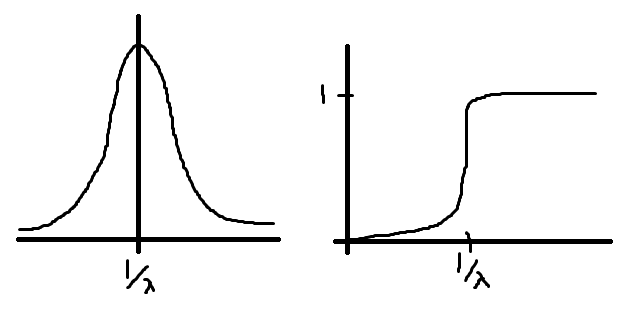
\includegraphics[width=100mm]{31.png}
		\caption{PDF and CDF for $\frac{S_n}{n}$}
	\end{figure}
	
	As $n\to\infty$, we see that
	
	\[\lim_{n\to\infty} F_n(x)=\begin{cases} 0 & x<1/\lambda \\ 1 & x>1/\lambda \end{cases}\]
	
	\begin{figure}[H]
		\centering
		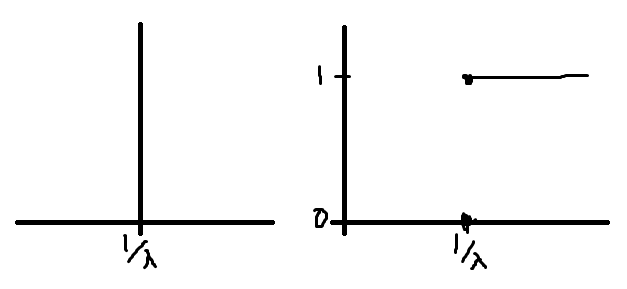
\includegraphics[width=100mm]{32.png}
		\caption{PDF and CDF for $\frac{S_n}{n}$ as $n\to\infty$}
	\end{figure}
\end{texample}

\begin{texample}
	Suppose a random variable $X_n$ is uniform on $\{\frac1n, \frac2n, \dots, \frac{n}{n}\}$. As $n\to\infty$, its CDF will look like the CDF for $\Unif(0, 1)$.
	
	\begin{figure}[H]
		\centering
		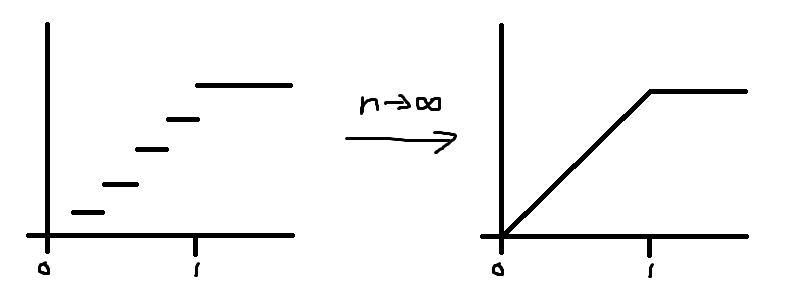
\includegraphics[width=100mm]{33.png}
		\caption{CDFs for $X_n$}
	\end{figure}
\end{texample}

If a random variables $X_n$ with CDF $F_n$ have $F_n\Rightarrow F$, we say that $X_n$ \textit{converge} in distribution:

\[X_n\xrightarrow{D}X\]

if $X$ has CDF $F$. In other words, $F_{X_n}(x)\Rightarrow F_X(x)$ whenever $F_X$ continuous.

\begin{theorem}
	Continuity Theorem: If random variables $X_n$ with CDF $F_n$ and characteristic function $\phi_n(t)$, then $\phi_n(t)\to\phi(t)$. If $\phi_n(t)\to\phi(t)$ for all $t$ and $\phi(t)$ is continuous at $0$, then $\phi(t)$ is the characteristic function of $X$ and $X_n\xrightarrow{D}X$.
\end{theorem}

\begin{texample}
	Continuing from the $\frac{S_n}{n}$ example, we saw that
	
	\[\lim_{n\to\infty} \phi_{\frac{S_n}{n}}(t)=e^{\frac{it}{\lambda}}\]
	
	By continuity theorem,
	
	\[\frac{S_n}{n}\xrightarrow{D}\frac{1}{\lambda}\]
	
	That is, the CDF of $\frac{S_n}{n}$ approximates to CDF of constant $\frac{1}{\lambda}$ (see figure 34). \\
	
	So, $P(a<\frac{S_n}{n}<b)=P(a<\frac{1}{\lambda}<b)$. In other words, the average of $X_1, X_2, \dots, X_n$ is approximately $\frac{1}{\lambda}$ with high probability.
\end{texample}

\begin{theorem}
	Weak Law of Large Numbers: Let $X_1, X_2, \dots, X_n$ be iid. random variables with the same distribution. Let the expectation for each random variable $X_i$, $\mu=EX_i$ is finite. Let $S_n = \sum_{i=1}^n X_i$, then
	
	\[\frac{S_n}{n} \xrightarrow{D} \mu\]
\end{theorem}
\begin{proof}
	By continuity theorem, it suffices to show that
	
	\[\lim_{n\to\infty} \phi_{\frac{S_n}{n}}(t)=e^{it\mu}\]
	
	for all $t$. We know that
	
	\[\phi_{\frac{S_n}{n}}(t)=\left( \phi_X\left( \frac{t}{n} \right) \right)^n\]
	
	Applying Taylor's expansion on $\phi_X$ about $t=0$ gives:
	
	\[\phi_X(s)=1+s\phi_X'(0)+O(s^2)=1+i(EX)s+O(s^2)\]
	
	Substituting this result into $\phi_X\left( \frac{t}{n} \right)$ gives
	
	\[\phi_X\left( \frac{t}{n} \right)=1+\frac{it\mu}{n}+O\left(\frac{t^2}{n^2}\right)\]
	
	Finally,
	
	\[\lim_{n\to\infty} \phi_{\frac{S_n}{n}}(t)= \lim_{n\to\infty} \left( 1+\frac{it\mu}{n}+O\left(\frac{t^2}{n^2}\right) \right)^n=e^{it\mu}\]
\end{proof}

Note that the continuity theorem needs the assumption that $\phi$ is continuous at $0$ otherwise $\phi$ will not be characteristic function of any random variable. As an example, consider the following characteristic function for $\Unif(-n,n)$:

\[\phi_n(t)=\begin{cases} \frac{\sin(nt)}{nt} & t \ne 0 \\ 1 & t = 0 \end{cases}\]

As $n\to\infty$,

\[\phi_n(t)=\begin{cases} 0 & t \ne 0 \\ 1 & t = 0 \end{cases}\]

This is not the characteristic function since it is discontinuous.

\subsection{Central Limit Theorem}

Consider an experiment where a fair coin is tossed $n$ times. The number of heads can be modelled with a binomial random variable $X\sim\Bin(n,1/2)$. Its PMF is

\[p(k)={n \choose k} \left( \frac12 \right)^n\]

\begin{figure}[H]
	\centering
	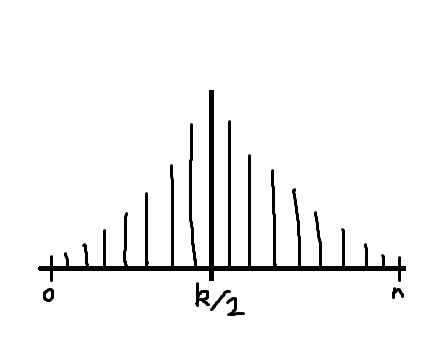
\includegraphics[width=100mm]{35.png}
	\caption{Distribution for Coin Tosses}
\end{figure}

The distribution looks almost like a bell curve. Let's see if we can transform the PMF into normal PDF. We start by applying Stirling's approximation $n!\approx\sqrt{2\pi n}\left(\frac{n}{e}\right)^n$.

\[p(k)=\frac{\sqrt{2\pi n}\left(\frac{n}{e}\right)^n}{\sqrt{2\pi k}\left(\frac{k}{e}\right)^k \sqrt{2\pi (n-k)}\left(\frac{n-k}{e}\right)^{n-k} 2^n}\]

When $k=\frac{n}{2}$,

\[p\left(\frac{n}{2}\right)\approx\frac{1}{\sqrt{\pi n}}\]

We introduce a parameter $t$ which denotes variation from $\frac{n}{2}$. So when $k=\frac{n}{2}+t$,

\[p\left(\frac{n}{2}+t\right)\approx\frac{1}{\sqrt{\pi n}}\exp\left( -\frac{t^2}{2n} \right)\]

This is a normal approximation which is valid when $n\gg 1$ and $t\ll n$. Poisson random variable also has the similar approximation:

\[p(\lambda + t)=\frac{1}{\sqrt{2\pi\lambda}}\exp\left( -\frac{t^2}{2\lambda} \right)\]

\begin{theorem}
	Central Limit Theorem (CLT): Let $X_1, X_2, \dots, X_n$ be iid. random variables, each with finite expectation $\mu=E[X_i]$ and finite variance $\sigma^2=\Var(X_i)$. Let $\bar{X}_n=\frac{1}{n}\sum_i X_i$ be the sample mean and $Z_n=\frac{\bar{X}_n - \mu}{\sigma/\sqrt{n}}$ or $Z_n=\frac{S_n - n\mu}{\sigma\sqrt{n}}$ where $S_n=X_1+X_2+\cdots+X_n$. Then we have
	
	\[Z_n\xrightarrow{D}\Norm(0,1)\]
	
	That is, as $n\to\infty$,
	
	\[P\left( a \le Z_n \le b \right) = \frac{1}{\sqrt{2\pi}} \int_a^b \exp\left(-\frac{x^2}{2}\right) dx\]
	
	for all $a$ and $b$.
\end{theorem}

\begin{proof}
	We start by defining a new random variable $Y_i=\frac{X_i-\mu}{\sigma}$ such that
	
	\[\sum_{i=1}^n \frac{Y_i}{\sqrt{n}}=Z_n\]
	
	$Y_i$ has zero expectation $E[Y_i]=0$ and unit variance $\Var(Y_i)=1$. By continuity theorem, it suffices to show that
	
	\[\phi_{Z_n}(t)\to e^{-\frac{t^2}{2}}\]
	
	as $n\to\infty$.
	
	\[\phi_{Z_n}(t)=\phi_{Y_1}\left(\frac{t}{\sqrt{n}}\right)\phi_{Y_2}\left(\frac{t}{\sqrt{n}}\right)\cdots \phi_{Y_n}\left(\frac{t}{\sqrt{n}}\right)=\left[\phi_{Y_i}\left(\frac{t}{\sqrt{n}}\right)\right]^n\]
	
	Applying Taylor's expansion on $\phi_{Y_i}\left(\frac{t}{\sqrt{n}}\right)$ gives:
	
	\[\phi_{Y_i}\left(\frac{t}{\sqrt{n}}\right)=1+\frac{it}{\sqrt{n}}E[Y_i]+\frac{i^2t^2}{2n}E[Y_i^2]+O(t^3)=1-\frac{t^2}{2n}+O(t^3)\]
	
	Finally,
	
	\[\lim_{n\to\infty} \phi_{Z_n}(t)=\lim_{n\to\infty} \left[1-\frac{t^2}{2n}+O(t^3)\right]^n=e^{-\frac{t^2}{2}}\]
\end{proof}

Remarks: If $EX_i=\infty$ or not defined then $\bar{X}_n$ has no limit. If $EX_i$ is defined but $\Var(X_i)=\infty$ then $\bar{X}_n \to \mu$ but $|\bar{X}_n - \mu| \gg 1/\sqrt{n}$.

\begin{texample}
	UBC wants to have $50$ new students in a certain program this year. Historically, only $40\%$ of admitted students accept the offer. If $100$ students admitted, what is the probability that more than $50$ people accept the offer? \\
	
	We can model the number of students who accepted the offer using a binomial random variable $X\sim\Bin(100,0.4)$. We need to find $P(X>50)$. \\
	
	We observe that $X$ is the sum of $100$ Bernoulli random variables with paramater $p=0.4$. The mean and variance for each Bernoulli random variable are $\mu=p=0.4$ and $\sigma^2=p(1-p)=0.24$. \\
	
	We define a new random variable $Z$:
	
	\[Z=\frac{X-np}{\sqrt{np(1-p)}}=\frac{X-40}{\sqrt{24}}\]
	
	By CLT, $Z$ can be approximated using standard normal $\Norm(0,1)$. So,
	
	\[P(X>50)=P\left(Z>\frac{50-40}{\sqrt{24}}\right)=P(Z>2.04)=1-\phi(2.04)\]
\end{texample}
